\documentclass{article}
\usepackage{graphicx}
\begin{document}
\section*{The Linux operating system}
Welcome to Linux. If you don't like it, it will make you:\newline
\begin{figure}[h]
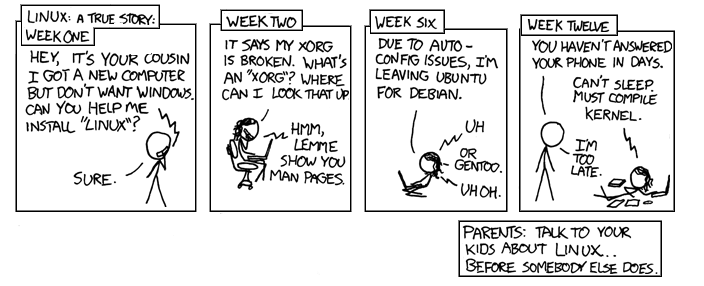
\includegraphics[height=120pt]{../pictures/xkcd_linux.png}
\end{figure}
\newline \\
You are running Xubuntu - a lightweight version of the popular Linux distribution -
Ubuntu. Here are some Linux basics to get you started:
\newline
\\ Note: To bring up the terminal, type \texttt{windows-key + T} or click on the
terminal icon on the bottom panel.
\section*{Terminology}
\begin{itemize}
\item In Linux, `folders' are called \emph{directories}.
\item The \emph{terminal} is a command line interface that makes seemingly difficult
		tasks easy.
\end{itemize} 
\section*{Navigating directories}
\begin{itemize}
\item \texttt{pwd} - Print working directory - default or \emph{home} is \texttt{/home/scicomp}
\item \texttt{cd path/to/directory} - Change directory
\newline
\\ example : \texttt{cd /home/scicomp/Documents}
\item \texttt{ls} - List all files and folders in directory
\end{itemize}
\section*{Python related}
\begin{itemize}
\item \texttt{python} - Start the Python shell
\item \texttt{python helloworld.py} - Run a python script named \texttt{helloworld.py}
			in the current directory
\end{itemize}
\end{document}
